% !TeX root = scaffold-50.tex
\renewcommand{\imagepath}{../50-unsupervised/img}
\newcommand{\ntopics}{n_\text{topics}}

\chapter{Unsupervised Analysis: Topic Modelling}
In this chapter, the topics of the celebrity newspaper articles are examined using the topic modelling technique. After showing that using \gls{lda} alone does not yield robust and reliable results, semantic-similarity clustering is shown to improve the quality of the topic extraction.  Finally, the significance of differences in the topic distributions of low-\gls{ses} and high-\gls{ses} newspaper articles are discussed.

The main focus is to find the prevailing topics in the celebrity newspaper articles and to examine any differences in the distribution of these topics between the low-\gls{ses} and high-\gls{ses} groups.\todo{Motivate more again}

\section{Shortcomings of \gls{lda} Topic Modelling}
In a first attempt, \gls{lda} model instances (see chapter~\ref{ch:lda}) were trained for a varying number of topics $\ntopics$. The corpus of all relevant newspaper articles comprised the 50-article balanced data set ensuring that role models with many articles could not induce a topic bias in the models. The texts were fed to the models in the \textit{noun and verb} stage in order to focus on the meaning-bearing elements of the texts.

Each of these model instances yielded a set of $\ntopics$ topics. Each topic $t$ is defined by a list $T_{\ntopics, t}$ of characterizing topic words. Each model assigned to every newspaper article $i$ estimated probabilities $p_{i, t}$ that article $i$ would belong to the topic $t$. Each newspaper article $i$ was assigned a topic $t_i$ by selecting the topic with the maximum probability:
\begin{align}
    t_i = \arg \max_{t'} p_{i, t'}
\end{align}

Figure~\ref{fig:topic_modelling_schema} illustrates the modelling and assigment process.
\begin{figure}
    \centering
    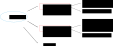
\includegraphics[]{\imagepath/topic_modelling_schema.pdf}
    \caption{Schematic of the topic modelling setup with \gls{lda}: Many models for different numbers $\ntopics$ of topics are trained, each of them yields a list of topics that are characterized by topic words, as well as topic probabilities for each article.}\label{fig:topic_modelling_schema}
\end{figure}

Sensible values for the model hyperparameters (except $\ntopics$) were found by trial and error. The following steps were taken to search for an optimal number of topics.\todo{Motivate more, why we look for n and what advantages and disadvantages a high and a low n have.}

\paragraph{Assigning Hypertopics}
As the topics are only defined by a list of characterizing words, the individual topics can semantically overlap, and topics which are output by different model instances cannot directly be compared. In order to still be able to compare the model outputs for different $n_\text{topics}$, each topic was manually assigned one of the four \textit{hypertopics} movie, music, sport, and life (with life being intended as a miscellaneous category for all topics not covered by the other three hypertopics). Each article $i$ with topic $t$ was by that means also assigned a hypertopic $h$:
\begin{align}
    h_i = h(t_i)
\end{align}

With every article associated to a hypertopic, it is possible to compare the distribution of articles and \gls{ses} groups across hypertopics for different $\ntopics$ as well as verifying topic assignments with the human-annotated data.

\paragraph{Accuracy and Consistency}
In the next step, the accuracy of the topic models was assessed with the human-annotated data and the consistency of the predictions for different $\ntopics$.

The accuracy of the hypertopic assignment was calculated as the ratio of artciles with correct hypertopic assigment by the model and all articles that were human-annotated:
\begin{align}
    acc = \frac{
        \left|
            \left\{i\middle|h_{i}^\text{predicted} = h_{i}^\text{true}\right\}
        \right|
    }{
        \left|
            \{{i|i \text{ was human-annotated}}\}
        \right|
    }
\end{align}

Figure~\ref{fig:accuracy_by_ntopics} reveals that the accuracy is not steady across different $\ntopics$ and comparably low.

\begin{figure}
    \centering
    \caption{Accuracy of the model-assigned hypertopics as a function of the number of topics: The accuracy of comparably low and not consistent across the different numbers of topics.}\label{fig:accuracy_by_ntopics}
\end{figure}

Additionally, the share of low-\gls{ses} articles for each assigned hypertopic was scrutinized in order to assess the influence of $\ntopics$ in the modelling quality. This share is plotted in figure~\ref{fig:lowshare_per_ntopics} across $\ntopics$. The fact that there is no range of $\ntopics$ where this share is consistent for small variations of $\ntopics$ suggests, that the assignment of articles to the hypertopics is to a large extent random and that the model is incapable of making a reliable prediction of an article's topic.\todo{Explain more why you took exactly this share and not anything else.}

\begin{figure}
    \centering
    \caption{Share of low-\gls{ses} articles in each hypertopic across different numbers of topics: The share is not consistent over a range from \SI{5}{} to \SI{50}{} topics, indicating that the assigment of articles to topics is not reliable.}\label{fig:lowshare_per_ntopics}
\end{figure}







\section{Improvement with Semantic Embeddings}

\section{Discussion}